\documentclass[11pt]{article}
\usepackage[margin=0.9in]{geometry}
\usepackage{amsmath,amssymb}
\usepackage{enumitem}
\usepackage{hyperref}
\usepackage{titlesec}
\usepackage{xcolor}
\usepackage{graphicx}
\usepackage{float}
\usepackage{array}
\usepackage{multirow}
\usepackage{fancyhdr}
\usepackage{tikz}

\usetikzlibrary{shapes,arrows,positioning,calc}

% Header/Footer
\pagestyle{fancy}
\fancyhf{}
\rhead{Team Egress}
\lhead{AI-Powered Timeline Travel Planning}
\cfoot{\thepage}

% Hyperlink setup
\hypersetup{
    colorlinks=true,
    linkcolor=blue!60!black,
    urlcolor=blue!60!black,
    citecolor=blue!60!black
}

% Section formatting
\titleformat{\section}{\Large\bfseries\color{blue!70!black}}{\thesection.}{0.5em}{}
\titleformat{\subsection}{\large\bfseries}{\thesubsection.}{0.5em}{}
\titleformat{\subsubsection}{\normalsize\bfseries}{\thesubsubsection.}{0.3em}{}

% Spacing
\setlength{\parindent}{0pt}
\setlength{\parskip}{0.6\baselineskip}
\setlist[itemize]{topsep=0.2em,itemsep=0.15em,leftmargin=1.3em}
\setlist[enumerate]{topsep=0.2em,itemsep=0.15em,leftmargin=1.5em}

\title{{\Large\bfseries AI-Powered Timeline Travel Planning Platform}\\
{\normalsize 12-Hour Development Report}\\
{\small Team Egress}}
\author{}
\date{June 21, 2026}

\begin{document}

\maketitle

\begin{abstract}
This report documents the development of an AI-powered travel planning platform that models trips as dynamic timelines with intelligent disruption handling, personalized recommendations, and cultural awareness. The system uses a multi-agent architecture to coordinate travel planning, logistics, real-time disruption response, and cultural guidance. The interim implementation delivers end-to-end architecture, microservices, web UI, and integration patterns for Sri Lanka-focused travel.
\end{abstract}

\tableofcontents
\newpage

% ============= SECTION 1: EXECUTIVE SUMMARY =============
\section{Executive Summary}

This project develops an intelligent travel assistant that transforms travel planning from static itineraries into a living, adaptive timeline. The platform represents a trip as a sequence of time-aware nodes (transport, accommodation, activities, meals, cultural sites, emergencies) that can be monitored, adapted, and optimized in real-time.

\textbf{Key Innovation:} A Trip Orchestrator Agent coordinates four specialized agents (Planner, Logistics, Disruption, Culture \& Etiquette) to manage the entire traveler journey, with automatic delay propagation and conflict detection across timeline dependencies.

\textbf{Target Domain:} Sri Lanka travel, capturing coastal routes, mountain passes, temples, wildlife parks, cultural sites, and weather-sensitive activities.

\textbf{12-Hour Deliverables:}
\begin{itemize}
    \item Complete system architecture (6 microservices + frontend)
    \item End-to-end LangGraph-based agent orchestration framework
    \item Database schema and domain service layer
    \item Web/mobile UI with timeline visualization
    \item Docker deployment infrastructure
    \item API Gateway with authentication
\end{itemize}

% ============= SECTION 2: PROBLEM & SOLUTION =============
\section{Problem Statement}

Travel planning today is fragmented:
\begin{itemize}
    \item Information scattered across 10+ platforms (maps, bookings, weather, events, cultural guides)
    \item Static itineraries that break when real-world changes occur
    \item No automatic propagation of delays to downstream activities
    \item Generic recommendations missing user context and preferences
    \item Cultural guidance absent (dress codes, temple etiquette, photography rules)
    \item No unified view of transport, lodging, activities, meals, and risks
\end{itemize}

For Sri Lanka—with coastal routes, mountain passes, temple visits, festivals, and unpredictable weather—this fragmentation is especially costly, leading to missed bookings, rushed travel, and cultural missteps.

\subsection{Solution: Timeline-Based Agentic Platform}

The platform represents a trip as a \textbf{time-ordered sequence of actionable nodes}. Each node contains:
\begin{itemize}
    \item \textbf{Operational:} start/end times, location, duration, transport method
    \item \textbf{Logistical:} booking IDs, confirmation details, transfer info
    \item \textbf{Cultural:} etiquette, dress code, photography rules, festival impacts
    \item \textbf{Contextual:} weather forecast, emergency contacts, risk indicators
    \item \textbf{Personal:} preferences, dietary needs, accessibility requirements
\end{itemize}

A \textbf{Trip Orchestrator Agent} receives user requests and coordinates \textbf{four specialized agents}:

\begin{table}[h]\centering\small
\begin{tabular}{|l|p{3.5in}|}
\hline
\textbf{Agent} & \textbf{Responsibility} \\
\hline
Planner & Builds itinerary; optimizes activity sequencing; recommends attractions, dining, timing \\
\hline
Logistics & Evaluates transport options; computes routes; manages transfer dependencies \\
\hline
Disruption & Handles delays, closures, weather; propagates impacts to dependent nodes; proposes recovery \\
\hline
Culture \& Etiquette & Supplies temple rules, dress codes, photography restrictions, festival guidance \\
\hline
\end{tabular}
\end{table}

When a traveler reports a delay (e.g., traffic to Kandy), the Disruption Agent estimates impact, checks conflicts (hotel check-in, dinner booking, temple visit, train), and proposes solutions (reschedule later nodes, substitute activity, take alternate route).

% ============= SECTION 3: SYSTEM ARCHITECTURE =============
\section{System Architecture}

\subsection{Layered Design}

The platform follows strict separation:

\begin{enumerate}
    \item \textbf{User Channels:} Web/Mobile app, WhatsApp/Telegram bot
    \item \textbf{API Gateway:} Request routing, authentication, rate limiting
    \item \textbf{Agentic Backend:} Trip Orchestrator + 4 specialized agents
    \item \textbf{Domain Services:} 7 specialized services (optimization, routing, weather, culture, alerts, notifications)
    \item \textbf{Shared State:} Trip DB (PostgreSQL), Vector DB (Qdrant for embeddings)
    \item \textbf{External APIs:} Weather, Maps/Routing, Transport Feeds, Tourism Content, News Alerts
\end{enumerate}

Key rule: \textbf{Agents call domain services; domain services call external APIs}. No direct external calls from agents.

\subsection{Microservices}

\begin{table}[H]\centering\small
\begin{tabular}{|l|p{2.8in}|p{1.2in}|}
\hline
\textbf{Service} & \textbf{Responsibility} & \textbf{Stack} \\
\hline
AI Service & LangGraph orchestration, vector retrieval, LangSmith tracing & Python, FastAPI \\
\hline
Trip Service & Trips, itineraries, bookings, timeline state & Python, FastAPI, PostgreSQL \\
\hline
User Service & Identity, profiles, preferences & Python, FastAPI \\
\hline
Booking Service & Reservation management & Python, FastAPI \\
\hline
Destination Service & Attractions, events, dining, ratings & Python, FastAPI \\
\hline
Gateway & API routing, auth, rate limiting & Kong, PostgreSQL \\
\hline
\end{tabular}
\end{table}

\subsection{Data Layer}

\begin{itemize}
    \item \textbf{Trip DB (PostgreSQL):} Users, trips, timeline nodes, bookings, alerts
    \item \textbf{Vector DB (Qdrant):} Embeddings for preferences, travel style, similar trips, personalization
    \item \textbf{Route Graph (Neo4j):} Transport network, connections, reachability queries
    \item \textbf{Cache (Redis):} Session state, queue jobs, rate limiting
\end{itemize}

% ============= SECTION 4: ARCHITECTURE DIAGRAM (TikZ) =============
\section{System Architecture Diagram}

\begin{figure}[H]
\centering
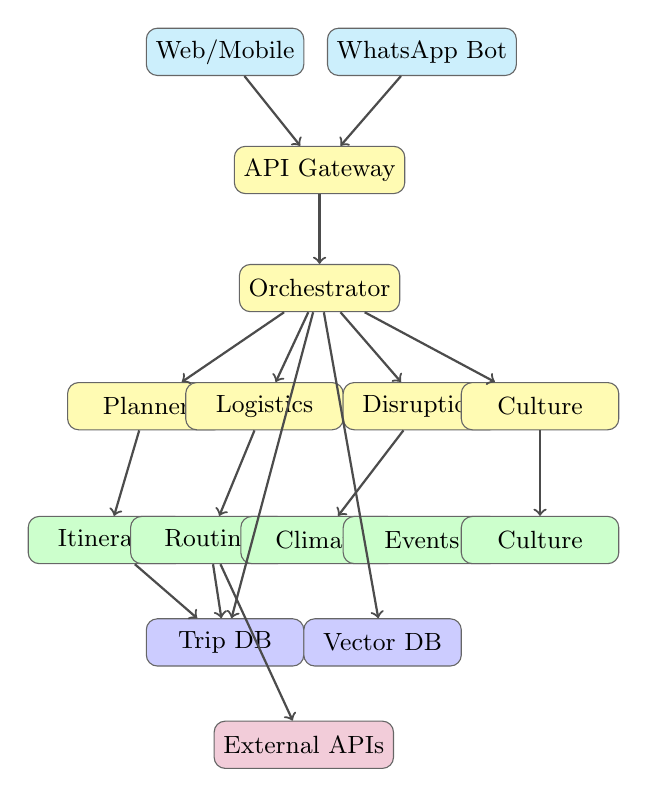
\begin{tikzpicture}[
  node distance=1.5cm,
  box/.style={rectangle, draw=black!60, fill=blue!10, rounded corners, minimum width=2cm, minimum height=0.6cm, font=\small},
  service/.style={rectangle, draw=black!60, fill=green!20, rounded corners, minimum width=2cm, minimum height=0.6cm, font=\small},
  external/.style={rectangle, draw=black!60, fill=purple!20, rounded corners, minimum width=2cm, minimum height=0.6cm, font=\small},
  arrow/.style={->, thick, black!70}
]

% User Layer
\node[box, fill=cyan!20] (web) at (0, 5) {Web/Mobile};
\node[box, fill=cyan!20] (bot) at (2.5, 5) {WhatsApp Bot};

% Gateway
\node[box, fill=yellow!30] (gw) at (1.2, 3.5) {API Gateway};

% Agents
\node[box, fill=yellow!30] (orch) at (1.2, 2) {Orchestrator};
\node[box, fill=yellow!30] (planner) at (-1, 0.5) {Planner};
\node[box, fill=yellow!30] (logistics) at (0.5, 0.5) {Logistics};
\node[box, fill=yellow!30] (disrupt) at (2.5, 0.5) {Disruption};
\node[box, fill=yellow!30] (culture) at (4, 0.5) {Culture};

% Domain Services
\node[service] (itin) at (-1.5, -1.2) {Itinerary};
\node[service] (route) at (-0.2, -1.2) {Routing};
\node[service] (climate) at (1.2, -1.2) {Climate};
\node[service] (events) at (2.5, -1.2) {Events};
\node[service] (cult-svc) at (4, -1.2) {Culture};

% Data Layer
\node[box, fill=blue!20] (tripdb) at (0, -2.5) {Trip DB};
\node[box, fill=blue!20] (vecdb) at (2, -2.5) {Vector DB};

% External
\node[external] (ext) at (1, -3.8) {External APIs};

% Connections
\draw[arrow] (web) -- (gw);
\draw[arrow] (bot) -- (gw);
\draw[arrow] (gw) -- (orch);
\draw[arrow] (orch) -- (planner);
\draw[arrow] (orch) -- (logistics);
\draw[arrow] (orch) -- (disrupt);
\draw[arrow] (orch) -- (culture);
\draw[arrow] (planner) -- (itin);
\draw[arrow] (logistics) -- (route);
\draw[arrow] (disrupt) -- (climate);
\draw[arrow] (culture) -- (cult-svc);
\draw[arrow] (orch) -- (tripdb);
\draw[arrow] (orch) -- (vecdb);
\draw[arrow] (itin) -- (tripdb);
\draw[arrow] (route) -- (tripdb);
\draw[arrow] (route) -- (ext);

\end{tikzpicture}
\caption{Simplified system architecture showing layered separation.}
\label{fig:architecture}
\end{figure}

% ============= SECTION 5: USE-CASE FLOWS =============
\section{Use-Case Flows}

\subsection{Primary Actors}
\begin{itemize}
    \item \textbf{Traveler:} Plans trips, views timeline, reports disruptions
    \item \textbf{System:} Proactive alert detection via external feeds
    \item \textbf{Admin:} Operates domain services, manages configuration
\end{itemize}

\subsection{Core Use Cases}

\begin{enumerate}
    \item \textbf{Create Trip Itinerary} — User provides dates, preferences, budget; Planner Agent generates initial timeline
    \item \textbf{View Timeline} — User opens trip and sees nodes (transport, stay, activity, meal) with state indicators
    \item \textbf{Preview Node} — User opens a node to see full details: route options, cultural notes, dining, emergency contacts
    \item \textbf{Report Delay} — User reports traffic, closure, or weather; Disruption Agent estimates impact
    \item \textbf{Automatic Delay Propagation} — System checks if delay conflicts with downstream reservations
    \item \textbf{Conflict Detection} — System highlights nodes affected by delay
    \item \textbf{Recovery Proposals} — System suggests: reschedule, substitute activity, take alternate route
    \item \textbf{Cultural Guidance} — User asks about temple etiquette; Culture Agent supplies rules and timing
    \item \textbf{Proactive Alert} — External feed signals event; system notifies user
    \item \textbf{Manage Preferences} — User updates budget, diet, transport; Vector DB stores for future personalization
\end{enumerate}

\subsection{Example Flow: Delay Handling}

\textit{``I'm stuck in traffic to Kandy—will I miss my 6 PM temple visit?''}

\begin{enumerate}
    \item Orchestrator identifies active node (transport to Kandy) and remaining timeline
    \item Disruption Agent estimates 45-minute delay
    \item System checks 6 PM temple node: requires 30-min walk + etiquette prep; arrival would be 5:55 PM (5 min risk)
    \item System flags conflict in timeline (temple node highlighted in red)
    \item Disruption Agent proposes: (a) reschedule temple to 7 PM, (b) visit alternative temple nearby, (c) extend dinner reservation
    \item User selects option; system validates feasibility (temple open 7 PM? transport available? dinner moved?)
    \item Timeline updates; system notifies user via push notification and SMS
\end{enumerate}

% ============= SECTION 6: ER MODEL =============
\section{Entity-Relationship Model}

\subsection{Core Entities}

\begin{table}[H]\centering\small
\begin{tabular}{|l|p{3.5in}|}
\hline
\textbf{Entity} & \textbf{Key Attributes} \\
\hline
User & id, email, phone, preferences (budget, diet, transport\_mode), created\_at \\
\hline
Trip & id, user\_id, start\_date, end\_date, destination, status (planning/active/completed) \\
\hline
Timeline Node & id, trip\_id, type (transport/stay/activity/meal/temple), start\_time, end\_time, location, state \\
\hline
Booking & id, node\_id, provider (hotel/airline/restaurant), confirmation\_id, status \\
\hline
Alert & id, trip\_id, node\_id, type (delay/closure/weather), severity, resolved\_at \\
\hline
Agent Run & id, trip\_id, agent (planner/logistics/disruption/culture), input, output, trace\_url \\
\hline
\end{tabular}
\end{table}

\subsection{Relationships}

\begin{itemize}
    \item User $\times$ Trip: One-to-Many (1 user $\rightarrow$ many trips)
    \item Trip $\times$ Timeline Node: One-to-Many (1 trip $\rightarrow$ many nodes)
    \item Timeline Node $\times$ Booking: One-to-Many (1 node $\rightarrow$ many bookings)
    \item Trip $\times$ Alert: One-to-Many (1 trip $\rightarrow$ many alerts)
    \item Trip $\times$ Agent Run: One-to-Many (1 trip $\rightarrow$ many orchestration runs)
\end{itemize}

% ============= SECTION 7: IMPLEMENTATION STATUS =============
\section{Implementation Status}

\subsection{Completed (\checkmark)}

\begin{itemize}
    \item Microservices architecture and Docker Compose setup
    \item API Gateway (Kong) with JWT authentication
    \item Core services: Trip, User, Booking, Destination
    \item Web UI (React + TypeScript) with timeline view, node details, settings
    \item LangGraph framework and agent state machine
    \item Domain service interfaces and patterns
    \item External API integration architecture
\end{itemize}

\subsection{In Progress (\textasciitilde)}

\begin{itemize}
    \item Full LangGraph agent node implementations
    \item Qdrant vector DB integration
    \item Neo4j route graph
    \item Real external API connections (currently mock data)
    \item Delay propagation logic and conflict detection
    \item Proactive alerts pipeline
\end{itemize}

\subsection{Backlog}

\begin{itemize}
    \item Multi-language support (Sinhala, Tamil)
    \item Push notifications and real-time updates
    \item Machine learning for personalization
    \item Native iOS/Android apps
    \item Advanced constraint solver for complex itineraries
\end{itemize}

% ============= SECTION 8: KEY DELIVERABLES =============
\section{Key Deliverables}

\subsection{Codebase Structure}

\begin{table}[H]\centering\small
\begin{tabular}{|l|l|}
\hline
\textbf{Component} & \textbf{Location} \\
\hline
Microservices (6) & \texttt{services/} \\
API Gateway & \texttt{gateway/} \\
Frontend (React) & \texttt{client/} \\
Infrastructure & \texttt{infra/} \\
Documentation & \texttt{docs/} \\
Diagrams & \texttt{diagram/}, \texttt{docs/} \\
\hline
\end{tabular}
\end{table}

\subsection{Deployment}

\begin{itemize}
    \item Docker Compose with 8+ services (PostgreSQL, Redis, Qdrant, Neo4j, Kong, etc.)
    \item Single command: \texttt{docker-compose up -d}
    \item Environment configs for dev, staging, production
    \item Monitoring: Grafana + Loki for logs and metrics
\end{itemize}

% ============= SECTION 9: TECHNICAL DECISIONS =============
\section{Technical Decisions}

\begin{enumerate}
    \item \textbf{Microservices:} Independent scaling, team ownership, technology choice per domain
    \item \textbf{Strict Layering:} Agents $\rightarrow$ Domain Services $\rightarrow$ External APIs. Prevents coupling, improves testability
    \item \textbf{LangGraph:} Control flow, state management, checkpointing; avoids ad-hoc async coordination
    \item \textbf{Vector DB:} Enables implicit context (infer active trip from session); improves over time
    \item \textbf{Neo4j:} Complex graph queries for transport connectivity and reachability
    \item \textbf{PostgreSQL:} Strong consistency for bookings, timelines, conflict detection
\end{enumerate}

% ============= SECTION 10: NEXT STEPS =============
\section{Next Steps}

\begin{enumerate}
    \item Complete LangGraph agent implementations with full tool bindings
    \item End-to-end integration testing: plan trip $\rightarrow$ report delay $\rightarrow$ propagate $\rightarrow$ recover
    \item Real external API connections (weather, transport, tourism)
    \item Embeddings pipeline and personalization testing
    \item Performance optimization and load testing
    \item User testing and feedback on timeline UX
    \item Cultural content validation with expert sources
\end{enumerate}

% ============= SECTION 11: CONCLUSION =============
\section{Conclusion}

This project delivers a novel approach to travel planning by modeling trips as dynamic, adaptive timelines managed by intelligent agents. The strict layered architecture, microservices design, and LangGraph orchestration provide a scalable foundation. The interim implementation demonstrates the core innovation: automatic delay propagation, conflict detection, and context-aware recovery recommendations.

With completion of agent logic, external API integration, and user testing, the platform can move toward production and expansion to other destinations.

\vspace{0.8cm}
\noindent\textbf{Project:} AGENTRIX26-TEAM02-Team\_Egress | \textbf{Deployment:} Docker Compose | \textbf{Date:} June 21, 2026

\end{document}